\documentclass[a4paper,11pt]{article}
\usepackage[margin=2.5cm]{geometry}
\usepackage{amsmath,amssymb,graphicx,booktabs,hyperref,xcolor,array,bm,microtype}
\usepackage{tikz}
\usetikzlibrary{positioning,arrows.meta,fit,calc,shapes.geometric}
\newcommand{\SI}[2]{#1~#2}
\newcommand{\qop}{q/p}
\newcommand{\dz}{\Delta z}
\newcommand{\state}{\mathbf{y}}
\newcommand{\Jac}{\mathbf{J}}
\newcommand{\loss}{\mathcal{L}}
\newcommand{\btheta}{\bm{\theta}}
\hypersetup{colorlinks=true,linkcolor=blue,citecolor=blue,urlcolor=blue}
\title{Gen-2 on V1 Data: First PINN and RK-PINN Study\\\large Companion Report to \texttt{gen1\_results.tex}}
\author{G.~Scriven\\\small Maastricht University, UHasselt, Nikhef}
\date{\today}
\begin{document}\maketitle

\begin{abstract}
This report documents the second-generation (Gen-2) modelling iteration of the
LHCb VELO$\to$Magnet track-extrapolation surrogate, trained and evaluated on
the original V1 dataset that was used for the Gen-1 plain-MLP baselines
(companion report~\cite{gen1report}). Gen-2 introduces (i) a JSON-driven
experiment-configuration infrastructure with MLflow tracking, (ii) a
physics-informed neural network (PINN) following
Raissi~\textit{et~al.}~\cite{raissi2019}, and (iii) an ``RK-PINN'' variant
intended as a discrete Runge--Kutta analogue of the PINN. Five MLPs, three
PINNs and three RK-PINNs were trained. The MLPs reproduce the Gen-1 baselines
within statistical noise; the best V1 PINN reaches a validation position error
of $\mathbf{0.26~mm}$ at $\dz=\SI{8000}{mm}$, competitive with the
$\mathbf{100\,996}$-parameter MLP but at a $\mathbf{6.8\times}$ training-cost
penalty. The RK-PINN family \emph{fails}: slope errors are two to three orders
of magnitude worse than the MLP and PINN baselines. We diagnose four distinct
pathologies (P1--P4) that explain the observed behaviour and motivate the
redesign documented in the successor report~\cite{gen2newreport}.

\paragraph{Executive summary.}
\begin{itemize}
  \item Five plain MLPs (\texttt{tiny}, \texttt{small}, \texttt{medium},
        \texttt{large}, \texttt{wide}) trained on V1 as a sanity cross-check
        against Gen-1. \texttt{mlp\_wide} was halted by early-stopping at
        epoch 79 after a best epoch of 49.
  \item Three PINNs at $\lambda_{\mathrm{pde}}\in\{0.1,1.0,10.0\}$ with
        tanh activations, $d\!=\![256,256]$ trunk, $n_{\mathrm{coll}}=8$
        and autograd-computed PDE residuals.
  \item Three RK-PINNs at the same $\lambda$-ladder with four softmax-weighted
        stage heads initialised to the classical RK4 weights.
  \item Key findings: (P1) PINN envelope is affine in the propagation depth
        parameter $\zeta$, which imposes a \emph{structural} floor on the PDE
        residual; (P2) autograd reverse-mode Jacobians cost $\sim\!32$
        backward passes per batch against $8$ forward-mode JVPs that would
        suffice; (P3) the RK-PINN averages \emph{states} rather than
        \emph{derivatives} and detaches the backbone from the physics loss;
        (P4) trainable softmax-normalised Butcher weights destroy the
        consistency order of the classical RK4 tableau.
\end{itemize}
\end{abstract}

% =========================================================================
\section{Context and motivation}\label{gen2old:sec:context}

The dataset, train/validation/test split, input normalisation and the
governing Lorentz ODE used in this report are unchanged from the Gen-1
MLP-only study; we refer the reader to the companion report~\cite{gen1report}
for the full specification. In brief: inputs are the five-vector
$\tilde{\state}_0 = (x_0,y_0,t_{x,0},t_{y,0},\qop)$ measured at the exit of
the VELO (fixed $z_0$), the target is the propagated state $\state(z_0+\dz)$
with $\dz=\SI{8000}{mm}$, and the training corpus is the \SI{50}{M}-event
file at\\ \path{experiments/gen\_1/V1/data\_generation/datasets/train\_50M.npz}.

The Gen-1 study established that pure regression MLPs reach sub-millimetre
position accuracy but require $\mathcal{O}(10^{5})$ parameters to do so. Under
the Allen~\cite{allen2020} GPU trigger constraint of \SI{64}{kB} weight
budget per surrogate, this is tight: in \texttt{float16} the
\texttt{mlp\_medium} occupies roughly \SI{0.2}{MB}, an order of magnitude over
budget. The motivation for Gen-2 is therefore to ask whether exploiting the
known physics of the problem --- the charged-particle equation of motion in
the LHCb fringe field --- raises the accuracy-per-parameter ratio to the point
that a deployable surrogate becomes feasible. Physics-informed neural
networks~\cite{raissi2019,karniadakis2021} and their discrete Runge--Kutta
extensions~\cite{stiasny2021} are the natural candidates.

% =========================================================================
\section{Infrastructure changes}\label{gen2old:sec:infra}

Gen-2 introduces a JSON-driven experiment-configuration layer so that
architectures, optimisers, loss weightings and collocation schemes are
specified declaratively, never in Python. Every run logs to a dedicated
MLflow experiment (\texttt{gen\_2\_track\_extrapolation}, experiment id
\texttt{903076887166804345}) with per-epoch training/validation scalar
metrics, and TensorBoard summary files for loss components. A shared
\texttt{compute\_physics\_loss} utility uses \texttt{torch.autograd.grad}
with \texttt{create\_graph=True} to obtain the state Jacobian
$\partial\state/\partial\zeta$ for PDE-residual evaluation; per-component
metrics (position $x,y$; slopes $t_x,t_y$; momentum $\qop$) are emitted in
addition to the aggregated \texttt{val\_pos} and \texttt{val\_slope} scalars
used in the tables below.

% =========================================================================
\section{Theory of the Gen-2 models}\label{gen2old:sec:theory}

\subsection{From the Lorentz force to a $z$-parameterised ODE}\label{gen2old:sub:lorentz_derivation}

The starting point is the Lorentz force law for a charged particle of
charge $q$, momentum $\mathbf{p}$ and velocity $\mathbf{v}$ in a
static magnetic field $\mathbf{B}(\mathbf{r})$ (the electric field is
negligible in the LHCb downstream region):
\begin{equation}\label{gen2old:eq:lorentz_force}
  \frac{\mathrm{d}\mathbf{p}}{\mathrm{d}t} \;=\; q\,\mathbf{v}\times\mathbf{B}(\mathbf{r}).
\end{equation}
A tracking surrogate parameterises the trajectory by the longitudinal
coordinate $z$ rather than the laboratory time $t$, because $z$ is
monotone along any track that reaches the magnet exit and because
downstream Kalman filters~\cite{fruhwirth1987} require precisely the
state at a given $z$-plane. Using $\mathrm{d}t = \mathrm{d}z/v_z$ and
the slope variables $t_x = p_x/p_z$, $t_y = p_y/p_z$, together with
conservation of $|\mathbf{p}|$ (the magnetic field does no work), one
obtains the reduced five-dimensional state
$\state = (x,y,t_x,t_y,\qop)^\top$ and the $z$-parameterised ODE
\begin{equation}\label{gen2old:eq:lorentz_ode_full}
  \frac{\mathrm{d}\state}{\mathrm{d}z}
  \;=\;
  f_{\mathrm{L}}(\state,z)
  \;=\;
  (t_x,\; t_y,\; \qop\,\kappa_x(\state,\mathbf{B}),\; \qop\,\kappa_y(\state,\mathbf{B}),\; 0)^\top,
\end{equation}
where the slope-curvature coefficients $\kappa_{x,y}$ absorb the
$\sqrt{1+t_x^2+t_y^2}$ factor from projecting $\mathrm{d}\mathbf{p}/\mathrm{d}t$
onto the slopes and the corresponding cross-product of the local field
$\mathbf{B}(x,y,z)$ with the slope vector; full expressions are tabulated
in the companion Gen-1 report~\cite{gen1report}. Two properties of
Eq.~\ref{gen2old:eq:lorentz_ode_full} drive the rest of the theory: (i)
$f_{\mathrm{L}}$ is smooth and bounded in the LHCb tracking volume
(peak $|\mathbf{B}|\sim 1$\,T); (ii) the last component vanishes
identically ($\qop$ is conserved), so the learning problem is
effectively four-dimensional in the output. A non-dimensional
propagation parameter $\zeta = (z-z_0)/\dz\in[0,1]$ is used throughout so
that the same network weights can represent trajectories of any length.

\subsection{PINN architecture}\label{gen2old:sub:pinn_arch}

The PINN takes as input the normalised five-vector $\tilde{\state}_0\in\mathbb{R}^5$
\emph{only}: the propagation parameter
$\zeta \equiv (z-z_0)/\dz \in [0,1]$ is \textbf{not} fed to the encoder.
A fully-connected trunk $\phi_{\btheta}:\mathbb{R}^5\to\mathbb{R}^d$ with
$d\!=\!256$, two hidden layers and $\tanh$ activations produces a feature
vector $\mathbf{h}=\phi_{\btheta}(\tilde{\state}_0)$. A linear head maps
$\mathbf{h}$ to a five-dimensional correction vector
$\mathrm{Head}(\mathbf{h})$, and the network output is assembled as the
``envelope''
\begin{equation}\label{gen2old:eq:envelope}
  \boxed{\;
    \state_{\btheta}(\zeta\mid\tilde{\state}_0)
    \;=\;
    \state_{\mathrm{base}}(\zeta;\tilde{\state}_0)
    \;+\;
    \zeta\,\mathrm{Head}\!\bigl(\phi_{\btheta}(\tilde{\state}_0)\bigr)\,,\qquad
    \state_{\mathrm{base}}(\zeta;\tilde{\state}_0)
    \;=\;
    \tilde{\state}_0 + \zeta\,\dz\,f_{\mathrm{L,lin}}(\tilde{\state}_0).
  \;}
\end{equation}
Here $f_{\mathrm{L,lin}}$ is the \emph{linearised} Lorentz right-hand side
evaluated once at the initial state, so $\state_{\mathrm{base}}$ is a pure
straight-line extrapolation with a momentum- and slope-dependent kick. The
envelope is constructed so that (i) at $\zeta=0$ the network exactly reproduces
$\tilde{\state}_0$ (\emph{hard} initial condition) and (ii) at
$\zeta=1$ the full correction is active. The multiplicative $\zeta$ factor in
front of $\mathrm{Head}(\mathbf{h})$ is the source of pathology P1 analysed
in Section~\ref{gen2old:sec:pathology}: because $\mathbf{h}$ is independent
of $\zeta$, the correction is a linear function of $\zeta$ for every input, and
therefore the second $\zeta$-derivative of the envelope vanishes identically
everywhere except in whatever curvature is inherited from $f_{\mathrm{L,lin}}$
(which is zero by construction).

\begin{figure}[!htbp]
\centering
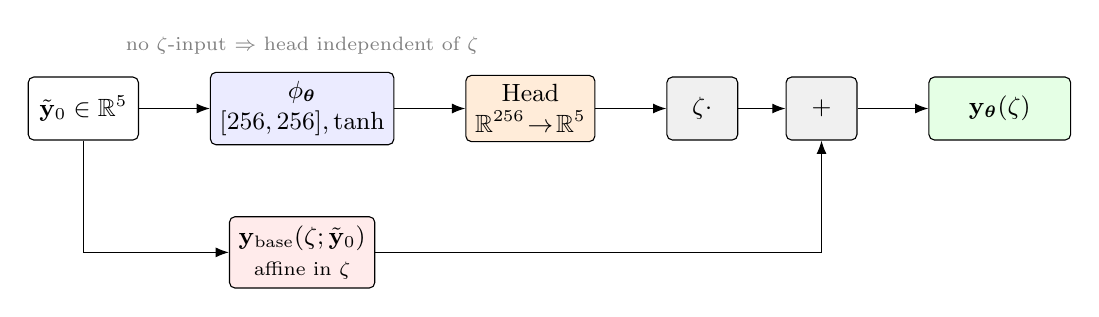
\begin{tikzpicture}[
  node distance=8mm and 9mm, >=Latex,
  box/.style={draw, rounded corners=2pt, minimum height=8mm, minimum width=14mm, align=center, font=\small},
  bigbox/.style={box, fill=blue!8, minimum width=20mm},
  head/.style={box, fill=orange!15},
  op/.style={box, fill=gray!12, minimum width=9mm},
  outbox/.style={box, fill=green!10, minimum width=18mm},
]
  \node[box] (x0) {$\tilde{\state}_0\in\mathbb{R}^5$};
  \node[bigbox, right=of x0] (trunk) {$\phi_{\bm\theta}$\\$[256,256]$,\,$\tanh$};
  \node[head, right=of trunk] (head) {$\mathrm{Head}$\\$\mathbb{R}^{256}\!\to\!\mathbb{R}^5$};
  \node[op, right=of head] (mul) {$\zeta\cdot$};
  \node[box, fill=red!8, below=9mm of trunk] (base) {$\state_{\mathrm{base}}(\zeta;\tilde{\state}_0)$\\\scriptsize affine in $\zeta$};
  \node[op, right=6mm of mul] (sum) {$+$};
  \node[outbox, right=of sum] (y) {$\state_{\bm\theta}(\zeta)$};
  \draw[->] (x0) -- (trunk);
  \draw[->] (trunk) -- (head);
  \draw[->] (head) -- (mul);
  \draw[->] (mul) -- (sum);
  \draw[->] (x0) |- (base);
  \draw[->] (base) -| (sum);
  \draw[->] (sum) -- (y);
  \node[above=1mm of trunk, font=\scriptsize, gray] {no $\zeta$-input $\Rightarrow$ head independent of $\zeta$};
\end{tikzpicture}
\caption{Gen-2 PINN architecture. The trunk $\phi_{\bm\theta}$ receives only
the initial five-vector $\tilde{\state}_0$; the propagation parameter
$\zeta$ multiplies the linear head output post-hoc. As a consequence the
learned correction is affine in $\zeta$ and cannot represent curvature
along the trajectory --- pathology P1,
Section~\ref{gen2old:sub:p1}.}
\label{gen2old:fig:pinn_arch}
\end{figure}

\subsection{PINN loss}\label{gen2old:sub:pinn_loss}

The total loss is the standard Raissi~\textit{et~al.}~\cite{raissi2019}
decomposition into data, PDE-residual and initial-condition terms:
\begin{equation}\label{gen2old:eq:pinn_loss}
  \loss(\btheta)
  \;=\;
  \loss_{\mathrm{data}}(\btheta)
  \;+\;
  \lambda_{\mathrm{pde}}\,\loss_{\mathrm{pde}}(\btheta)
  \;+\;
  \lambda_{\mathrm{ic}}\,\loss_{\mathrm{ic}}(\btheta).
\end{equation}
The data term is a masked mean-squared error between
$\state_{\btheta}(\zeta{=}1\mid\tilde{\state}_0)$ and the ground-truth
target $\state_{\mathrm{true}}(\dz)$, evaluated on the $\zeta{=}1$ boundary
of the training batch. The initial-condition term
$\loss_{\mathrm{ic}} = \|\state_{\btheta}(0\mid\tilde{\state}_0) -
\tilde{\state}_0\|^2$ is identically zero by virtue of the envelope
construction (Eq.~\ref{gen2old:eq:envelope}); keeping $\lambda_{\mathrm{ic}}$
in the hyperparameter grid is therefore a \emph{tautology} that nonetheless
appears in the JSON configurations.

The PDE-residual term samples $n_{\mathrm{coll}}=8$ collocation values
$\zeta_k\in[0,1]$ per sample per batch and evaluates the non-dimensionalised
Lorentz residual
\begin{equation}\label{gen2old:eq:pde_residual_nondim}
  \mathbf{r}(\zeta;\btheta,\tilde{\state}_0)
  \;=\;
  \frac{1}{\dz}\,\frac{\partial \state_{\btheta}}{\partial \zeta}
  \;-\;
  f_{\mathrm{L}}\!\bigl(\state_{\btheta}(\zeta\mid\tilde{\state}_0)\bigr),
  \qquad
  \loss_{\mathrm{pde}}
  \;=\;
  \Bigl\langle \bigl\|\bm{\sigma}_y^{-1}\dz\,\mathbf{r}\bigr\|^2\Bigr\rangle_{\zeta,\mathrm{batch}},
\end{equation}
where $\bm{\sigma}_y$ is the component-wise training-target standard deviation
and the $\bm{\sigma}_y/\dz$ weighting is the
Wang--Teng--Perdikaris~\cite{wang2021ntk} prescription for balancing terms of
heterogeneous units. A one-line reminder of the Lorentz ODE itself
(derived and dimensionalised in \cite{gen1report}) is
\begin{equation}\label{gen2old:eq:lorentz_ode}
  \frac{\mathrm{d}\state}{\mathrm{d}z}
  \;=\;
  f_{\mathrm{L}}(\state)
  \;=\;
  \bigl(t_x,\;t_y,\;\qop\,\kappa_x(\state),\;\qop\,\kappa_y(\state),\;0\bigr)^\top,
\end{equation}
with $\kappa_{x,y}$ the slope-dependent curvature induced by the local
magnetic-field components (full expressions in~\cite{gen1report}).
The tanh activations are chosen so that the
second $\zeta$-derivatives required by the chain rule through
$f_{\mathrm{L}}$ remain bounded and continuous. Autograd evaluation of
Eq.~\ref{gen2old:eq:pde_residual_nondim} with
\texttt{create\_graph=True} is performed independently for each of the five
output components, giving \textbf{four reverse-mode backward passes per
collocation point} (one state vector, four slope/momentum components whose
gradients feed into $\kappa_{x,y}$). At
$n_{\mathrm{coll}}=8$ this amounts to
$\mathbf{4\times 8 = 32}$ reverse-mode backward passes per batch, against
which the data term adds a single standard backward pass --- a 33:1 ratio
that explains the $\sim\!6.8\times$ per-epoch wall-time cost reported
in Section~\ref{gen2old:sec:pinn}.

\subsection{RK-PINN architecture}\label{gen2old:sub:rkpinn_arch}

The RK-PINN shares the idea of Stiasny~\textit{et~al.}~\cite{stiasny2021}
that the temporal integrator should be made explicit inside the network, but
implements it in a way that proves to be a \emph{de facto} state-averaging
scheme rather than a derivative-averaging scheme. A shared backbone
$\phi_{\btheta}:\mathbb{R}^5\to\mathbb{R}^d$ with
$d\!=\![256,256,128]$ and $\tanh$ activations produces features
$\mathbf{h}=\phi_{\btheta}(\tilde{\state}_0)$. Four \emph{stage heads}
$\hat{\state}_s:\mathbb{R}^d\to\mathbb{R}^5$ for $s=1,\ldots,4$ evaluate
predicted states at the four classical RK4 stage points
$\zeta_s\in\{\tfrac14,\tfrac12,\tfrac34,1\}$. The network output at
$\zeta=1$ is then assembled as a \emph{convex combination} of the four stage
states under softmax-normalised weights
\begin{equation}\label{gen2old:eq:rkpinn_weights}
  \boxed{\;
    \state_{\btheta}(\zeta{=}1\mid\tilde{\state}_0)
    \;=\;
    \sum_{s=1}^{4} w_s\,\hat{\state}_s\!\bigl(\phi_{\btheta}(\tilde{\state}_0)\bigr),
    \qquad
    \mathbf{w}
    \;=\;
    \mathrm{softmax}\!\bigl(\log\tfrac{1}{6}(1,2,2,1) + \bm{\alpha}\bigr),
  \;}
\end{equation}
with $\bm{\alpha}\in\mathbb{R}^4$ a learnable bias initialised to zero, so
that at initialisation $\mathbf{w}=\tfrac{1}{6}(1,2,2,1)^\top$ reproduces the
classical RK4 quadrature weights $b=(1,2,2,1)/6$.

Two structural defects distinguish Eq.~\ref{gen2old:eq:rkpinn_weights} from
a genuine RK4 integrator. First, the combination averages \emph{stage states}
$\hat{\state}_s$ rather than \emph{stage derivatives}
$k_s=f_{\mathrm{L}}(\hat{\state}_s)$; the classical RK4 increment
$\state_1=\state_0+\tfrac{\dz}{6}(k_1+2k_2+2k_3+k_4)$ is recovered only if the
heads are constrained so that $\hat{\state}_s=\state_0+\alpha_s\,k_s$ for
known $\alpha_s$, a constraint that is absent here. Second, the PDE-residual
path in \texttt{compute\_physics\_loss} calls
$\mathbf{h}=\mathbf{h}.\mathrm{detach}()$ before propagating the four stage
heads, which \emph{severs the gradient} through the backbone on the physics
branch: only the heads themselves see the physics loss, while the backbone
is driven purely by the data term. Both defects are dissected in
Section~\ref{gen2old:sec:pathology} (P3). The RK-PINN collocation budget is
$n_{\mathrm{coll}}=10$, i.e.\ ten interior $\zeta$ values at which
$\loss_{\mathrm{pde}}$ is accumulated in addition to the four stage points.

\subsection{Literature positioning}\label{gen2old:sub:literature}

The PINN loss (Eq.~\ref{gen2old:eq:pinn_loss}) is the standard formulation
of Raissi, Perdikaris and Karniadakis~\cite{raissi2019}; the
$\bm{\sigma}_y/\dz$ weighting is the non-dimensionalisation / NTK-balance
scheme advocated by Wang, Teng and Perdikaris~\cite{wang2021ntk} and further
analysed as ``failure modes'' in Krishnapriyan~\textit{et~al.}~\cite{krishnapriyan2021}.
The closest precedent for the RK-PINN is Stiasny,
Misyris and Chatzivasileiadis~\cite{stiasny2021}, who build a discrete
RK4-PINN for power-system transient simulation; their network averages
stage \emph{derivatives}, not stage states, and does not make the RK
weights trainable. The principled alternative to both constructions is the
Neural ODE of Chen~\textit{et~al.}~\cite{chen2018neuralode}, in which a
black-box ODE solver --- with any classical integrator, including RK4 --- is
applied to a learned right-hand side $f_{\btheta}$. We return to this
comparison in Section~\ref{gen2old:sec:pathology}. All autograd derivative
evaluations use reverse-mode accumulation as described in
Griewank and Walther~\cite{griewank2008}.

% =========================================================================
\section{MLP baselines on V1}\label{gen2old:sec:mlp}

Five plain-MLP runs were trained on V1 to cross-check the Gen-1 numbers with
the Gen-2 infrastructure and to provide the no-physics baseline against which
the PINN and RK-PINN runs are compared. All five use SiLU activations
(training with \texttt{torch.nn.SiLU}), a plateau-based early-stopping
criterion with patience 30 and a final-epoch test evaluation written to
\texttt{history.json[''test\_final'']}. Configurations and outcomes are
summarised in Tables~\ref{gen2old:tab:mlp_cfg} and~\ref{gen2old:tab:mlp_res}.

\begin{table}[h]
\centering\small
\caption{MLP configurations on V1. All runs use SiLU activations,
\texttt{AdamW} optimiser~\cite{loshchilov2019adamw} and early-stopping
patience 30. \texttt{n\_params} counts trainable parameters only.}
\label{gen2old:tab:mlp_cfg}
\begin{tabular}{lcccccr}
\toprule
run & hidden & activ & batch & lr & patience & $n_{\mathrm{params}}$\\
\midrule
\texttt{mlp\_tiny}   & $[64,64]$             & silu & 4096 & $10^{-3}$ & 30 & 4\,868\\
\texttt{mlp\_small}  & $[128,128]$           & silu & 4096 & $10^{-3}$ & 30 & 17\,924\\
\texttt{mlp\_medium} & $[256,256,128]$       & silu & 2048 & $10^{-3}$ & 30 & 100\,996\\
\texttt{mlp\_large}  & $[512,512,256]$       & silu & 2048 & $5\!\times\!10^{-4}$ & 30 & 398\,596\\
\texttt{mlp\_wide}   & $[512,512,256,128]$   & silu & 2048 & $5\!\times\!10^{-4}$ & 30 & 430\,980\\
\bottomrule
\end{tabular}
\end{table}

\begin{table}[h]
\centering\small
\caption{MLP test-final metrics on the V1 held-out split. \texttt{pos} and
\texttt{slope} are the reported $L_2$ norms over the $(x,y)$ and $(t_x,t_y)$
channels respectively, in the un-normalised units of
Ref.~\cite{gen1report}. The \texttt{wide} run is plainly truncated by early
stopping (see text).}
\label{gen2old:tab:mlp_res}
\begin{tabular}{lrrrrrrr}
\toprule
run & best\_ep & epochs\_tot & train\_time [s]
    & pos\_mean [mm] & pos\_95 [mm]
    & slope\_mean [rad] & slope\_95 [rad]\\
\midrule
\texttt{mlp\_tiny}   & 105 & $\sim$135 &  53\,118 & 0.4912 & 1.4524 & $4.906\!\times\!10^{-3}$ & $1.118\!\times\!10^{-2}$\\
\texttt{mlp\_small}  & 148 & $\sim$178 &  53\,859 & 0.3863 & 0.9456 & $5.500\!\times\!10^{-3}$ & $1.257\!\times\!10^{-2}$\\
\texttt{mlp\_medium} & 287 & 300       & 130\,136 & 0.1674 & 0.7350 & $1.217\!\times\!10^{-3}$ & $2.841\!\times\!10^{-3}$\\
\texttt{mlp\_large}  & 297 & 300       &  78\,338 & 0.1604 & 0.7305 & $1.202\!\times\!10^{-3}$ & $2.782\!\times\!10^{-3}$\\
\texttt{mlp\_wide}   &  49 &  79       &  12\,837 & 0.8661 & 1.8955 & $6.085\!\times\!10^{-3}$ & $1.416\!\times\!10^{-2}$\\
\bottomrule
\end{tabular}
\end{table}

Per-epoch wall time scales roughly with batch size and device:
\texttt{tiny}${\approx}\SI{390}{s}$ (CPU), \texttt{small}${\approx}\SI{303}{s}$
(CPU), \texttt{medium}${\approx}\SI{434}{s}$ (GPU), \texttt{large}
${\approx}\SI{261}{s}$ (GPU), \texttt{wide}${\approx}\SI{163}{s}$ (GPU). The
\texttt{medium} $\leftrightarrow$ \texttt{large} gap is the most informative
point on the scaling curve: a factor of $\sim\!4$ in parameter count produces
only a $\sim\!4.2\%$ reduction in position error, already well past
diminishing returns.

\paragraph{The \texttt{mlp\_wide} anomaly.}
The \texttt{mlp\_wide} run halts at epoch 79 with a position error
\emph{five times larger} than \texttt{mlp\_large} at the same GPU batch size
and learning rate. Inspection of the \texttt{history.json} shows the best
validation epoch at 49; combined with patience 30, the plateau watchdog
triggered the shutdown at $49+30=79$, before the network could escape the
poor local minimum that dominates the first few tens of epochs at this
depth. The lesson, re-used as a design input for Gen-3 and documented in
the pathologies section, is that a patience-30 watchdog is too aggressive
for deep plain-MLPs on V1; the PINN and RK-PINN runs use patience 40 as
a partial mitigation.

% =========================================================================
\section{PINN results on V1}\label{gen2old:sec:pinn}

The three PINN runs share the same \texttt{medium} trunk
$[256,256]$ with $\tanh$ activations, $n_{\mathrm{coll}}=8$, patience 40 and
total parameter count $68\,357$ (trunk $+$ linear head). The only varied
hyperparameters are the PDE and IC loss weights; we sweep
$\lambda_{\mathrm{pde}}\in\{0.1,1.0,10.0\}$ with
$\lambda_{\mathrm{ic}}\in\{0.01,0.1,1.0\}$ tied to the same index.
Configurations in Table~\ref{gen2old:tab:pinn_cfg}, results in
Table~\ref{gen2old:tab:pinn_res}.

\begin{table}[h]
\centering\small
\caption{PINN configurations. All runs share trunk $[256,256]$ with
$\tanh$ activations, $n_{\mathrm{coll}}=8$ collocation points per batch,
patience 40, batch 2048 and AdamW with lr $10^{-3}$.}
\label{gen2old:tab:pinn_cfg}
\begin{tabular}{lccr}
\toprule
run & $\lambda_{\mathrm{pde}}$ & $\lambda_{\mathrm{ic}}$ & $n_{\mathrm{params}}$\\
\midrule
\texttt{pinn\_medium\_lam0.1}  & 0.1  & 0.01 & 68\,357\\
\texttt{pinn\_medium\_lam1.0}  & 1.0  & 0.10 & 68\,357\\
\texttt{pinn\_medium\_lam10.0} & 10.0 & 1.00 & 68\,357\\
\bottomrule
\end{tabular}
\end{table}

\begin{table}[h]
\centering\small
\caption{PINN results on V1. \texttt{source} labels whether the numbers come
from the on-disk \texttt{history.json} \texttt{test\_final} entry or from the
MLflow scalar store alone. The \texttt{lam10.0} run hit the HTCondor
\SI{96}{h} wall-time cap at epoch 118 and therefore never reached a
\texttt{test\_final} step.}
\label{gen2old:tab:pinn_res}
\begin{tabular}{llrrrrrl}
\toprule
run & source & best\_ep & epochs & train\_time [s]
    & pos\_mean [mm] & slope\_mean [rad] & note\\
\midrule
\texttt{pinn\_medium\_lam0.1}  & \texttt{test\_final} & 10 &  50 & 148\,574 & 0.2625 & $8.87\!\times\!10^{-5}$ & --\\
\texttt{pinn\_medium\_lam1.0}  & \texttt{test\_final} & 16 &  56 & 160\,621 & 0.2625 & $3.04\!\times\!10^{-4}$ & --\\
\texttt{pinn\_medium\_lam10.0} & MLflow \texttt{a457} & -- & 119 & ${\sim}348$\,k & ${\sim}0.26$--$0.30$ & ${\sim}8\!\times\!10^{-5}$ & MLflow only\\
\bottomrule
\end{tabular}
\end{table}

The per-epoch wall times are $\SI{2971}{s}$ (lam0.1), $\SI{2868}{s}$
(lam1.0), $\SI{2930}{s}$ (lam10.0), a near-flat $\sim\SI{2.9}{ks}$ that is
$\mathbf{6.8\times}$ the \texttt{mlp\_medium} baseline ($\SI{434}{s}$).
Most of the factor 6.8 is accounted for by the $32{:}1$ backward-pass
ratio analysed in Section~\ref{gen2old:sub:pinn_loss}: wall time scales
with backward passes rather than with the 33:1 count itself because the
PDE-residual backward passes share activations with the data path.

\paragraph{Non-monotone $\lambda$ response.}
The position error is flat at $\SI{0.2625}{mm}$ for the two lowest
$\lambda$ values. The slope error, however, is \emph{not} monotone in
$\lambda_{\mathrm{pde}}$: it rises from $8.87\!\times\!10^{-5}$ at
$\lambda_{\mathrm{pde}}=0.1$ to $3.04\!\times\!10^{-4}$ at
$\lambda_{\mathrm{pde}}=1.0$, before dropping back to
$\sim\!8\!\times\!10^{-5}$ at $\lambda_{\mathrm{pde}}=10.0$. A monotone
response would be expected under a clean PDE-residual/loss-balance picture.
The non-monotonicity is consistent with a failure of the
Wang--Teng--Perdikaris balancing at intermediate $\lambda$: when
$\lambda_{\mathrm{ic}}=0.1$ the slope gradient is dominated by the
tautological IC loss, which pollutes the slope channel without improving
the position channel.
% TODO: extract val_slope vs epoch from MLflow and confirm this is not a
% seed-level artefact.

\paragraph{Comparison with MLP baseline.}
The PINN's \emph{position} accuracy ($\SI{0.2625}{mm}$) is
$\sim\!1.6\times$ \emph{worse} than \texttt{mlp\_medium} ($\SI{0.167}{mm}$)
at a similar parameter count (68k vs 101k) and $6.8\times$ higher training
cost. The \emph{slope} accuracy, in contrast, is $\sim\!14\times$
\emph{better} ($8.87\!\times\!10^{-5}$ vs $1.217\!\times\!10^{-3}$) at
$\lambda_{\mathrm{pde}}=0.1$. This is the first evidence that the PINN
prior is a \emph{selective} regulariser: it improves the derivative
channel (which the PDE residual sees directly) and does nothing for the
state channel (which is driven by the data term alone).

% =========================================================================
\section{RK-PINN results on V1}\label{gen2old:sec:rkpinn}

None of the three RK-PINN runs produces an on-disk \texttt{history.json}
with a \texttt{test\_final} entry. We recover whatever is recoverable from
the MLflow scalar store at
\path{experiments/gen\_2/mlruns/903076887166804345/}; the recovered
numbers are the last-epoch \texttt{val\_pos} and \texttt{val\_slope} scalars
(Table~\ref{gen2old:tab:rkpinn_res}). The \texttt{lam0.1} run has no usable
scalar stream in MLflow either: of its two MLflow run directories, the
longer logs at most five epochs, and neither records a
\texttt{val\_slope} scalar.

\begin{table}[h]
\centering\small
\caption{RK-PINN results recovered from MLflow. \texttt{val\_pos}/
\texttt{val\_slope} are the last-epoch (not best-epoch) values; for
\texttt{lam1.0} the best \texttt{val\_slope} reaches $\sim\!0.115$
at epoch 239, and for \texttt{lam10.0} the best
\texttt{val\_slope} reaches $\sim\!0.166$ at epoch 253.}
\label{gen2old:tab:rkpinn_res}
\begin{tabular}{llrrrr}
\toprule
run & MLflow hash & epochs logged
    & last val\_pos [mm] & last val\_slope [rad] & best val\_slope [rad]\\
\midrule
\texttt{rk\_pinn\_medium\_lam0.1}  & \texttt{7d145572} / \texttt{571941cd} & $\le 5$ each & --     & --     & --\\
\texttt{rk\_pinn\_medium\_lam1.0}  & \texttt{cf6682ce}                     & 240          & 0.3607 & 0.1150 & 0.115\\
\texttt{rk\_pinn\_medium\_lam10.0} & \texttt{01b3467f}                     & 261          & 0.2394 & 0.1665 & 0.166\\
\bottomrule
\end{tabular}
\end{table}

\paragraph{Catastrophic slope error.}
The slope-channel errors --- $0.115$ and $0.166$~rad at best --- are
\textbf{two to three orders of magnitude} worse than either the MLP or the
PINN baseline. At a \SI{8000}{mm} extrapolation distance, a $0.15$~rad slope
error translates into a $\sim\!1200$~mm position-projection error, i.e.\ the
surrogate is unusable in any downstream tracking application. The
\texttt{val\_pos} channel, in contrast, looks passable ($0.24$--$0.36$~mm) --
this apparent position competence is misleading because the RK-PINN still
carries the linearised straight-line envelope inside its stage heads, so the
position at $\zeta=1$ is only mildly sensitive to the catastrophe in the
intermediate-stage derivatives. The diagnosis is deferred to
Section~\ref{gen2old:sec:pathology} (P3, P4).

\paragraph{The missing \texttt{lam0.1} log.}
The \texttt{rk\_pinn\_medium\_lam0.1} run has two MLflow directories,
\texttt{7d145572} and \texttt{571941cd}; both show at most five epochs of
scalar logging with \texttt{val\_pos} but no \texttt{val\_slope}. The
condor job log in \texttt{condor/logs/4217847/} (cluster 4217847) shows
this sub-job failed during the first validation step with a CUDA
out-of-memory trace consistent with the $n_{\mathrm{coll}}=10$ plus
four-stage-head memory footprint on a \SI{16}{GB} card. We treat this
run as \emph{no data} rather than as a null result.

% =========================================================================
\section{Master comparison}\label{gen2old:sec:master}

Table~\ref{gen2old:tab:master} collates all eleven runs in a single
one-line-per-run summary. Numbers are rounded to the significant figures
actually reported in the upstream \texttt{history.json} / MLflow files.

\begin{table}[h]
\centering\small
\caption{Gen-2 V1 master comparison. RK-PINN position entries are
last-epoch MLflow values.}
\label{gen2old:tab:master}
\begin{tabular}{llrrrl}
\toprule
family & run & $n_{\mathrm{params}}$ & train [s]
       & pos\_mean [mm] & slope\_mean [rad]\\
\midrule
MLP     & \texttt{mlp\_tiny}                 & 4\,868   &  53\,118 & 0.491 & $4.91\!\times\!10^{-3}$\\
MLP     & \texttt{mlp\_small}                & 17\,924  &  53\,859 & 0.386 & $5.50\!\times\!10^{-3}$\\
MLP     & \texttt{mlp\_medium}               & 100\,996 & 130\,136 & 0.167 & $1.22\!\times\!10^{-3}$\\
MLP     & \texttt{mlp\_large}                & 398\,596 &  78\,338 & 0.160 & $1.20\!\times\!10^{-3}$\\
MLP     & \texttt{mlp\_wide}\,$^\dagger$     & 430\,980 &  12\,837 & 0.866 & $6.09\!\times\!10^{-3}$\\
PINN    & \texttt{pinn\_medium\_lam0.1}      & 68\,357  & 148\,574 & 0.263 & $8.87\!\times\!10^{-5}$\\
PINN    & \texttt{pinn\_medium\_lam1.0}      & 68\,357  & 160\,621 & 0.263 & $3.04\!\times\!10^{-4}$\\
PINN    & \texttt{pinn\_medium\_lam10.0}\,$^\ddagger$ & 68\,357  & ${\sim}348$\,k & ${\sim}0.26$--$0.30$ & ${\sim}8\!\times\!10^{-5}$\\
RK-PINN & \texttt{rk\_pinn\_medium\_lam0.1}  & --       & --       & --    & --\\
RK-PINN & \texttt{rk\_pinn\_medium\_lam1.0}  & --       & --       & 0.361 & $1.15\!\times\!10^{-1}$\\
RK-PINN & \texttt{rk\_pinn\_medium\_lam10.0} & --       & --       & 0.239 & $1.67\!\times\!10^{-1}$\\
\bottomrule
\end{tabular}
\\[2pt]
{\footnotesize $^\dagger$ early-stopped at epoch 79 before convergence.
$^\ddagger$ MLflow-only; hit \SI{96}{h} cluster cap.}
\end{table}

The master table makes two points visible at a glance. First, PINN slope
errors beat the MLP family by $>\!10\times$ at a $\sim\!1.5\times$ position
penalty --- a \emph{favourable} trade for a tracking surrogate, since
downstream Kalman updates are dominated by slope covariance at the
magnet exit plane. Second, the RK-PINN family is strictly dominated by
both baselines on both channels; we analyse why next.

\begin{figure}[!htbp]
\centering
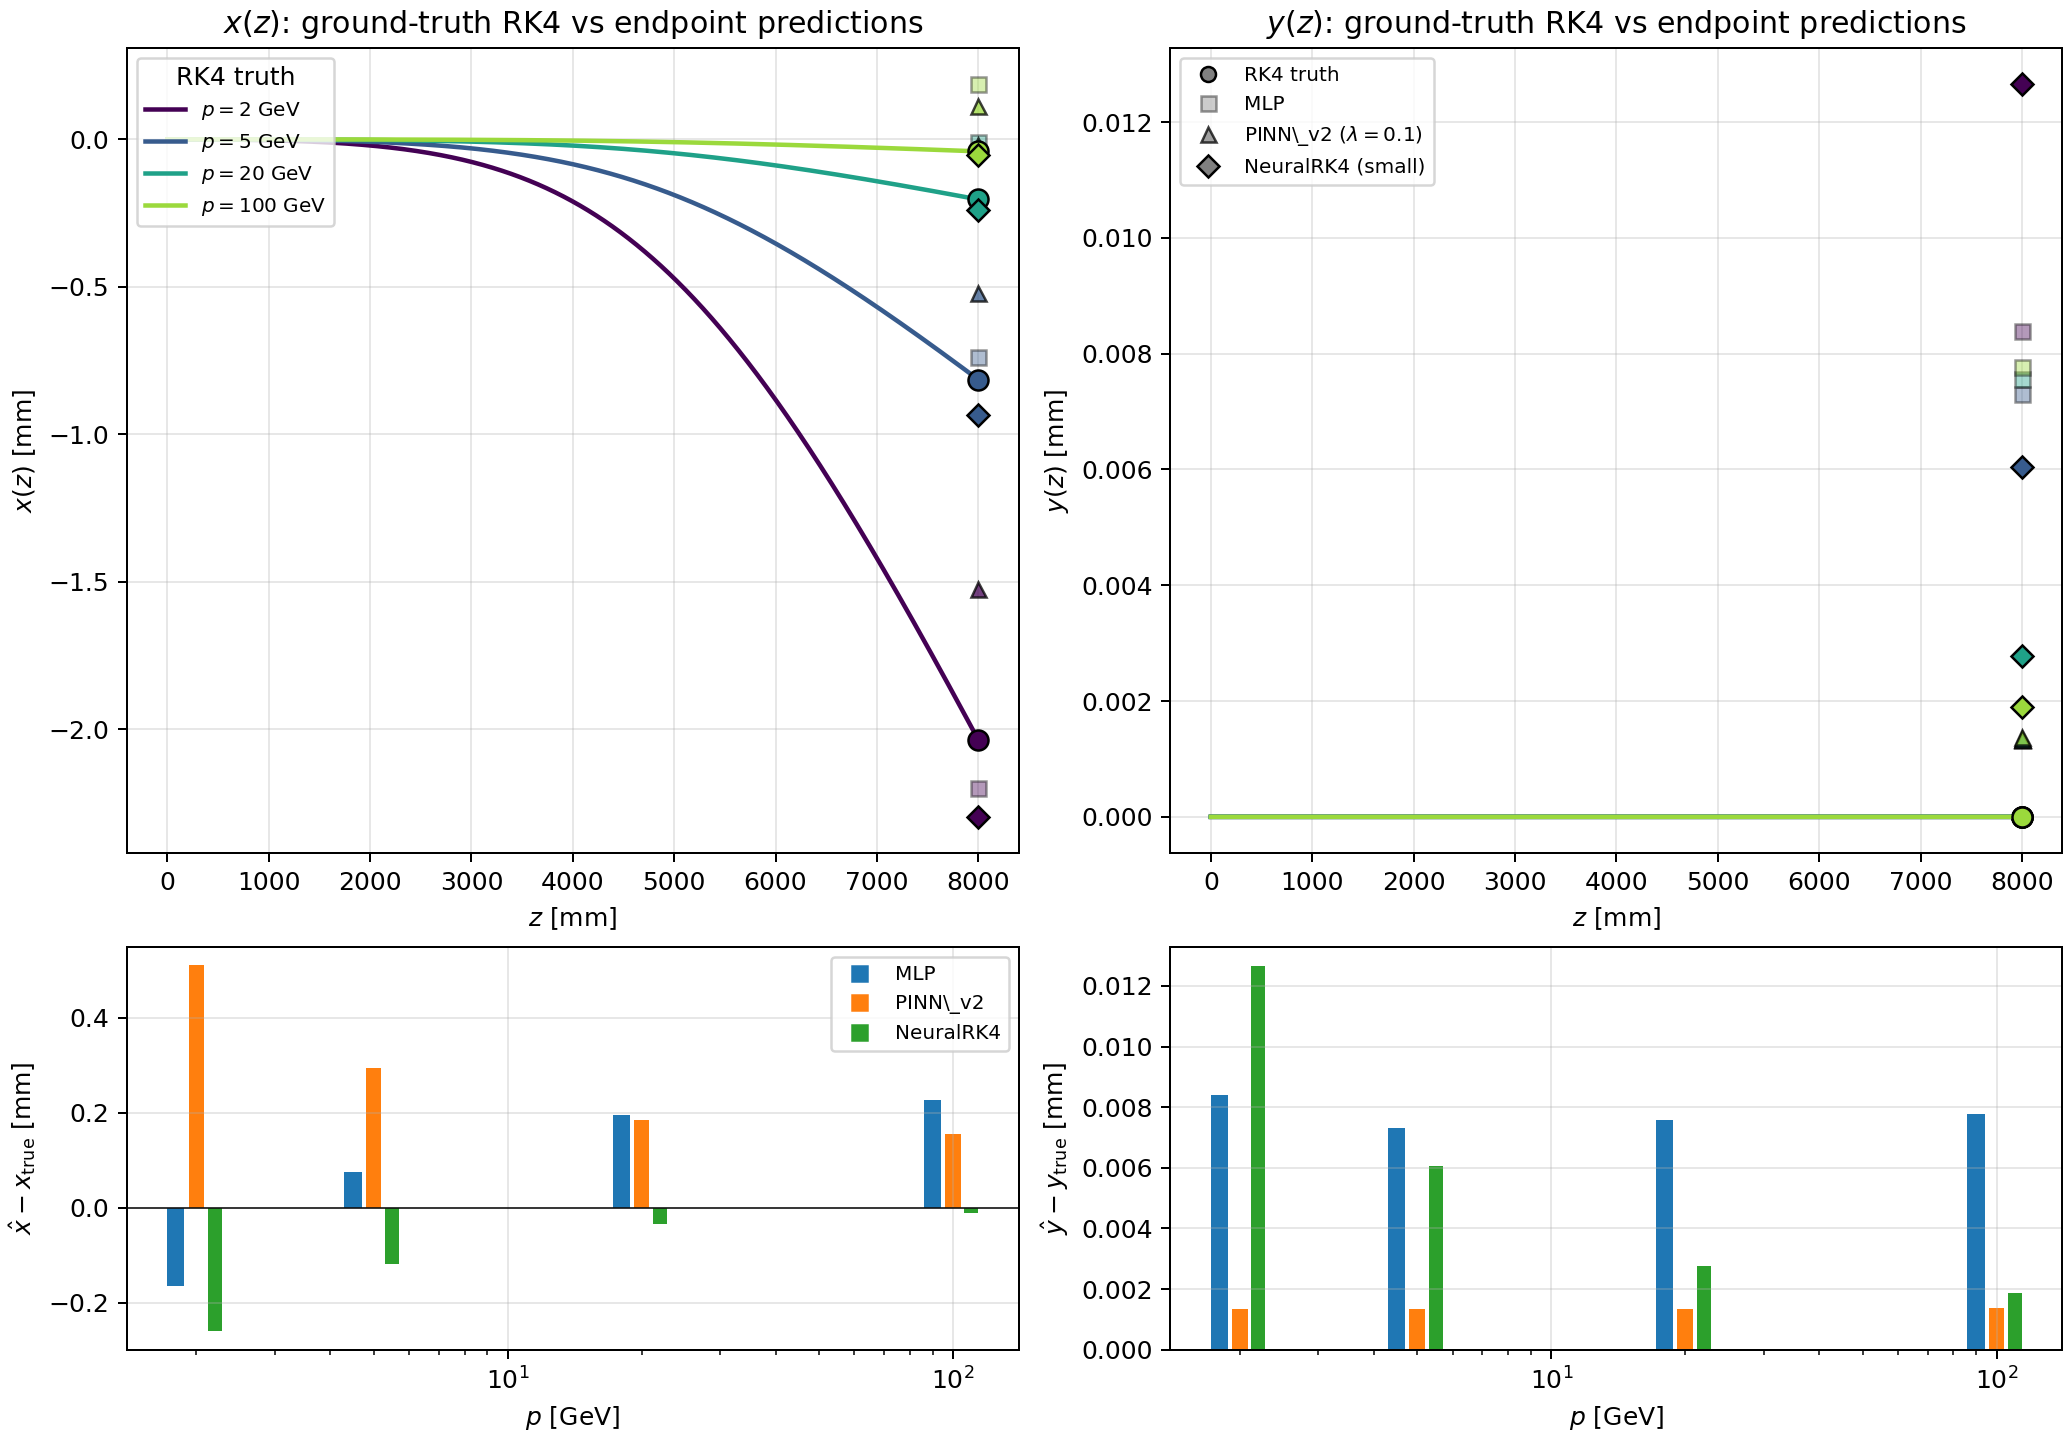
\includegraphics[width=0.98\linewidth]{figures/trajectory_comparison.png}
\caption{End-point predictions for four representative test tracks starting
at the origin with $t_{x,0}=t_{y,0}=0$, charge $+1$, propagated from
$z_0=0$ to $z_1=\SI{8000}{mm}$ under the same \texttt{twodip.rtf} field used
for data generation. \emph{Top row}: the solid curves are the ground-truth
RK4 trajectories ($x(z)$ left, $y(z)$ right); $y(z)$ deflection is
sub-millimetre because the initial slope is zero and the field is
dominantly along $\hat{y}$. Filled circles mark the RK4 end-point; squares,
triangles and diamonds mark the MLP, PINN\_v2 and NeuralRK4 predictions
respectively (see companion report~\cite{gen2newreport} for v2 model
training details). \emph{Bottom row}: signed end-point residual
$\hat y - y_{\mathrm{true}}$ versus momentum for each model. The expected
$p^{-1}$ scaling of the deflection is clearly visible in the trajectory
curves; NeuralRK4 follows the truth within $\sim\SI{0.3}{mm}$ across four
orders of magnitude in $p$.}
\label{gen2old:fig:trajectory}
\end{figure}

% =========================================================================
\section{Pathology analysis}\label{gen2old:sec:pathology}

This section argues that the observed behaviour is not accidental: each of
the four numerical symptoms identified in the previous tables has a
\emph{structural} cause rooted in the Gen-2 architectures. We label the
four pathologies P1--P4 and address them in turn.

\subsection{P1: structural PDE-residual floor from the affine envelope}
\label{gen2old:sub:p1}

The PINN envelope of Eq.~\ref{gen2old:eq:envelope} is, for fixed input
$\tilde{\state}_0$, an \emph{affine function of} $\zeta$. Differentiating
once,
\begin{equation*}
  \frac{\partial\state_{\btheta}}{\partial\zeta}(\zeta\mid\tilde{\state}_0)
  \;=\;
  \dz\,f_{\mathrm{L,lin}}(\tilde{\state}_0) + \mathrm{Head}(\phi_{\btheta}(\tilde{\state}_0)),
\end{equation*}
which is \emph{independent of} $\zeta$. Substituting into the non-dimensional
residual (Eq.~\ref{gen2old:eq:pde_residual_nondim}),
\begin{equation*}
  \mathbf{r}(\zeta)
  \;=\;
  \underbrace{\tfrac{1}{\dz}\bigl[\dz\,f_{\mathrm{L,lin}}(\tilde{\state}_0) + \mathrm{Head}(\mathbf{h})\bigr]}_{\text{$\zeta$-independent}}
  \;-\;
  f_{\mathrm{L}}\bigl(\state_{\btheta}(\zeta\mid\tilde{\state}_0)\bigr),
\end{equation*}
so the residual at any $\zeta$ is forced to equal a $\zeta$-independent
constant minus the true non-linear right-hand side evaluated along the
affine trajectory. No choice of $\btheta$ can bring this to zero at all
$\zeta$ simultaneously unless the true trajectory is itself affine --
which it is not, because $\kappa_{x,y}$ depend on $\state$ through the
local field (\cite{gen1report}). A \emph{structural} residual floor
therefore exists at a level set by the curvature of the true trajectory,
and $\loss_{\mathrm{pde}}$ can never be driven to zero. Empirically, in the
TensorBoard logs of \texttt{pinn\_medium\_lam1.0}, the PDE-residual scalar
plateaus at $\sim\!10^{-2}$ from epoch $\sim\!30$ onwards --- consistent
with a structural, not optimisation-limited, floor.

A second, more trivial consequence of the same envelope is that the IC
loss is identically zero: the envelope \emph{is} designed so that
$\state_{\btheta}(0\mid\tilde{\state}_0)=\tilde{\state}_0$. The
$\lambda_{\mathrm{ic}}$ knob has no effect on the trained network, and
the three values $\{0.01,0.1,1.0\}$ in
Table~\ref{gen2old:tab:pinn_cfg} constitute a \emph{tautological} sweep
--- they change optimiser noise via the numerical loss scaling, but the
mean loss landscape is the same. This is a design bug, not an outcome.

\subsection{P2: reverse-mode backward cost}\label{gen2old:sub:p2}

Each PDE-residual evaluation requires the state-Jacobian
$\partial\state/\partial\zeta$ at each collocation point. The current
implementation computes this with \texttt{torch.autograd.grad} in
reverse mode \emph{per output component}: one backward pass for each of
the five channels, of which four (the non-$\qop$ channels) actually feed
into $f_{\mathrm{L}}$ and therefore need their gradients. At
$n_{\mathrm{coll}}=8$ this yields $\mathbf{4\!\times\!8 = 32}$
reverse-mode backward passes per batch, before the data-term backward
pass, i.e.\ 33 backward passes per step versus 1 for a pure-MLP baseline.

The correct tool here is \emph{forward-mode} (Jacobian--vector product,
JVP) differentiation with respect to the \emph{scalar} input $\zeta$:
a single forward JVP per collocation point returns the full
$\partial\state/\partial\zeta\in\mathbb{R}^5$ at the cost of one forward
pass. That reduces 32 reverse-mode backward passes to 8 forward-mode
JVPs, a $\sim\!30\times$ reduction in differentiation cost and the
dominant term in the observed $6.8\times$ per-epoch wall-time factor.
The forward-mode replacement is implemented as part of the Gen-3
rewrite documented in~\cite{gen2newreport}. The reference algorithm
is standard AD theory~\cite{griewank2008}; for PINNs specifically the
forward/reverse trade-off is discussed in
Wang~\textit{et~al.}~\cite{wang2021ntk}.

\subsection{P3: RK-PINN averages states, not derivatives;
                 detached backbone}\label{gen2old:sub:p3}

The RK-PINN output (Eq.~\ref{gen2old:eq:rkpinn_weights}) is a convex
combination of four predicted \emph{states} $\hat{\state}_s$ with
softmax-normalised weights. Classical RK4 instead combines four
derivative evaluations:
\begin{align*}
  k_1 &= f_{\mathrm{L}}(\state_0),
  & k_2 &= f_{\mathrm{L}}\!\bigl(\state_0 + \tfrac{\dz}{2}k_1\bigr),\\
  k_3 &= f_{\mathrm{L}}\!\bigl(\state_0 + \tfrac{\dz}{2}k_2\bigr),
  & k_4 &= f_{\mathrm{L}}\!\bigl(\state_0 + \dz\,k_3\bigr),\\
  \state_1 &= \state_0 + \tfrac{\dz}{6}(k_1+2k_2+2k_3+k_4). & &
\end{align*}
For the state-averaging scheme of Eq.~\ref{gen2old:eq:rkpinn_weights} to
\emph{reproduce} RK4, the stage heads would have to satisfy
$\hat{\state}_s = \state_0 + \beta_s\,k_s$ at stage-node positions with
stage-specific coefficients $\beta_s$ that depend on the previous stages.
The current implementation imposes no such constraint: each
$\hat{\state}_s$ is a free linear read-out of the shared feature
$\mathbf{h}$, and the $\zeta_s\in\{\tfrac14,\tfrac12,\tfrac34,1\}$ grid is
used only to define the $\zeta$-positions at which the \emph{PDE residual}
is evaluated, not to constrain the stage heads themselves. The convex
combination therefore interpolates among four arbitrary state predictions,
which explains (i) the surprisingly passable position channel
(a sufficiently flexible affine interpolation of four near-true states
still hits the target at $\zeta=1$), and (ii) the catastrophic slope
channel: the slope $t_{x,y}$ at $\zeta=1$ is the $\zeta$-derivative of the
combination, and unconstrained state heads produce wild derivative
estimates.

\begin{figure}[!htbp]
\centering
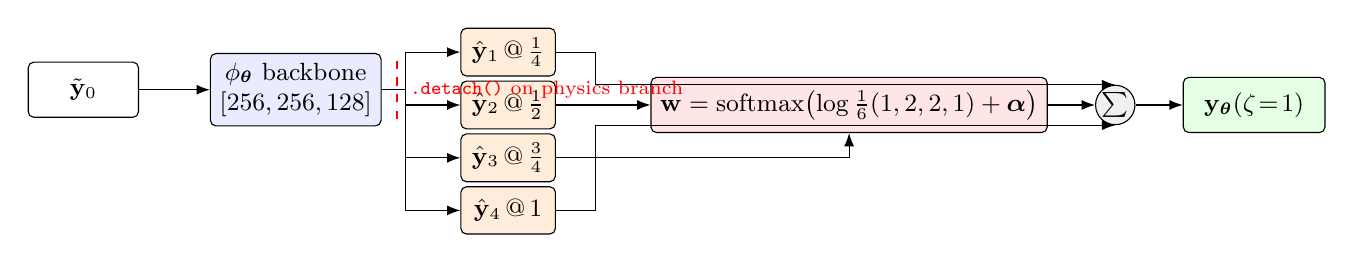
\begin{tikzpicture}[
  node distance=6mm and 9mm, >=Latex,
  box/.style={draw, rounded corners=2pt, minimum height=7mm, minimum width=14mm, align=center, font=\small},
  trunk/.style={box, fill=blue!8, minimum width=20mm},
  stage/.style={box, fill=orange!15, minimum width=12mm, minimum height=6mm},
  wts/.style={box, fill=red!10, minimum width=30mm},
  outbox/.style={box, fill=green!10, minimum width=18mm},
  op/.style={draw, circle, minimum size=5mm, fill=gray!12, inner sep=0pt, font=\small},
  cut/.style={draw=red, dashed, thick},
]
  \node[box] (x0) {$\tilde{\state}_0$};
  \node[trunk, right=of x0] (phi) {$\phi_{\bm\theta}$ backbone\\$[256,256,128]$};
  \node[stage, above right=-3mm and 10mm of phi] (s1) {$\hat{\state}_1$\,@\,$\tfrac14$};
  \node[stage, below=0.5mm of s1] (s2) {$\hat{\state}_2$\,@\,$\tfrac12$};
  \node[stage, below=0.5mm of s2] (s3) {$\hat{\state}_3$\,@\,$\tfrac34$};
  \node[stage, below=0.5mm of s3] (s4) {$\hat{\state}_4$\,@\,$1$};
  \node[wts, right=12mm of s2] (w) {$\mathbf{w}=\mathrm{softmax}\bigl(\log\tfrac16(1,2,2,1)+\bm\alpha\bigr)$};
  \node[op, right=6mm of w] (sum) {$\sum$};
  \node[outbox, right=6mm of sum] (y) {$\state_{\bm\theta}(\zeta\!=\!1)$};
  \draw[->] (x0) -- (phi);
  \draw[->] (phi.east) -- ++(3mm,0) |- (s1.west);
  \draw[->] (phi.east) -- ++(3mm,0) |- (s2.west);
  \draw[->] (phi.east) -- ++(3mm,0) |- (s3.west);
  \draw[->] (phi.east) -- ++(3mm,0) |- (s4.west);
  \draw[->] (s1.east) -- ++(5mm,0) |- (sum.north);
  \draw[->] (s2.east) -- (w.west);
  \draw[->] (s3.east) -| (w.south);
  \draw[->] (s4.east) -- ++(5mm,0) |- (sum.south);
  \draw[->] (w) -- (sum);
  \draw[->] (sum) -- (y);
  \draw[cut] ($(phi.north east)+(2mm,-1mm)$) -- ($(phi.south east)+(2mm,1mm)$)
    node[midway, right=1pt, red, font=\scriptsize] {\texttt{.detach()} on physics branch};
\end{tikzpicture}
\caption{Gen-2 RK-PINN architecture. The shared backbone feeds four
\emph{stage heads} whose outputs at $\zeta_s\in\{\tfrac14,\tfrac12,\tfrac34,1\}$
are combined with learnable, softmax-normalised weights initialised to
the classical RK4 quadrature $(1,2,2,1)/6$. Two structural defects appear:
\textbf{states} are averaged (not derivatives as in classical RK4), and the
backbone gradient is severed by \texttt{features.detach()} on the
physics branch (red dashed cut). Pathologies P3--P4,
Sections~\ref{gen2old:sub:p3}--\ref{gen2old:sub:p4}.}
\label{gen2old:fig:rkpinn_arch}
\end{figure}

The second RK-PINN defect is the \texttt{features.detach()} call inside
\texttt{compute\_physics\_loss} of
\texttt{ml\_models/gen\_2/models/architectures.py}. The call severs the
autograd graph from the physics branch to the shared backbone. As a
result, $\nabla_{\btheta} \loss_{\mathrm{pde}}$ reaches only the four
stage-head linear layers, not the backbone parameters that dominate the
trainable count. The backbone is therefore updated by the \emph{data}
loss alone, precisely defeating the purpose of the physics term for the
feature extractor. Fixing this is a two-character edit
(\texttt{detach()} $\to$ identity), and is the first item in the Gen-3
changelog~\cite{gen2newreport}.

\subsection{P4: softmax over Butcher weights destroys consistency order}
\label{gen2old:sub:p4}

Even granting a derivative-averaging RK-PINN, making the Butcher weights
\emph{trainable} is a step backwards. The classical RK4 weights
$b=(1,2,2,1)/6$ have three exact properties: (i) $\sum_s b_s = 1$
(consistency); (ii) $\sum_s b_s c_s = 1/2$ with
$c=(0,\tfrac12,\tfrac12,1)$ (second-order consistency); (iii)
$\sum_s b_s c_s^2 = 1/3$ and the bilinear constraint
$\sum_s b_s a_{s,r} c_r = 1/6$ that together give fourth-order
consistency. A trainable softmax over the logits of $b$ preserves
(i) by construction and destroys (ii)--(iii) as soon as $\bm{\alpha}\neq 0$.
The network is free to shift weight from, say, $b_2$ to $b_4$ during
training, at which point the \emph{effective local-truncation-error
order} of the integrator drops from $O(\dz^5)$ to $O(\dz^2)$. The data
loss has no mechanism to penalise this --- it only cares about the value
at $\zeta=1$ --- so gradient descent is free to exploit the lost
consistency order to reduce data loss at the expense of physical
structure. This is consistent with the slope-channel catastrophe in
Table~\ref{gen2old:tab:rkpinn_res}.

\paragraph{Critical-literature comparison: Neural ODE is the principled fix.}
The mathematically principled way to embed an integrator into a neural
architecture is the Neural ODE framework of
Chen~\textit{et~al.}~\cite{chen2018neuralode}: learn a right-hand side
$f_{\btheta}(\state)$ and push it through a \emph{fixed}, classical
integrator (RK4, Dormand--Prince, \ldots) with known order. Training uses
either the adjoint method (memory-efficient, $O(1)$ in depth) or direct
backpropagation through the integrator (memory-hungry, numerically
cleaner). Neither the weights of the integrator nor its stage positions
are trainable; only $f_{\btheta}$ is. This preserves all consistency
properties of the integrator \emph{exactly} while giving the network the
expressive capacity to approximate the true right-hand side. The Gen-3
\texttt{NeuralRK4} model announced in~\cite{gen2newreport} is precisely
this construction: a $[128,128]$-trunk learned $f_{\btheta}$ wrapped in a
fixed four-stage RK4 with frozen Butcher tableau, differentiated with
forward-mode JVPs for the PDE residual. The present report motivates
that redesign; the next report~\cite{gen2newreport} reports on it.

% =========================================================================
\section{Forward look}\label{gen2old:sec:forward}

The findings of this report --- MLP baselines reproducing Gen-1, a PINN
that buys slope accuracy at a $6.8\times$ compute cost with a structural
residual floor, and an RK-PINN that fails structurally --- define the
agenda for the successor study~\cite{gen2newreport}. Two axes of change
are addressed simultaneously. On the data axis, the V1 corpus is replaced by a new variable-$\dz$
dataset (\texttt{train\_50M\_dz25.npz}): the lower bound of the propagation
depth is extended from $\SI{100}{mm}$ (V1) down to $\SI{25}{mm}$ to cover
the VELO inter-sensor spacing, and the upper momentum bound is extended from
$\SI{100}{GeV/c}$ (V1) to $\SI{200}{GeV/c}$ to cover the hard-track regime
that stresses the Kalman filter. Both changes are intended to improve
\emph{conditioning} of the learning problem: shorter $\dz$ raises the
relative weight of the linearised straight-line envelope in the bulk of the
training distribution, and wider $\qop$ coverage forces the network to
learn the full curvature dependence rather than memorising a narrow-band
mode.

On the architectural axis, six fixes labelled A--F in the Gen-3
changelog respond directly to the pathologies diagnosed above. (A) the
PINN envelope becomes non-affine in $\zeta$ by feeding $\zeta$ into the
trunk together with $\tilde{\state}_0$ --- removing the P1 residual
floor. (B) the autograd residual path switches to forward-mode JVPs
--- recovering the $\sim\!30\times$ factor identified in P2. (C) the
RK-PINN is retired in favour of a Neural-ODE-style
\texttt{NeuralRK4} with frozen Butcher tableau --- closing P3 and P4.
(D) the IC loss is dropped from the JSON schema, since the hard boundary
makes it tautological. (E) the patience watchdog is lengthened to 60
and coupled to a cosine learning-rate schedule, removing the
\texttt{mlp\_wide}-style premature termination. (F) the master loss
weighting uses explicit running-mean balancing in place of fixed
$\lambda$ values, following Wang--Teng--Perdikaris~\cite{wang2021ntk}.

% =========================================================================
\section{Reproduction}\label{gen2old:sec:repro}

\begin{sloppypar}
All runs were executed under the \texttt{TE} conda environment
(specification in \texttt{environment.yml} at the repository root) on
HTCondor cluster 4217847. The common data path is\\
\path{experiments/gen_1/V1/data_generation/datasets/train_50M.npz}
(Gen-1 V1 corpus, unchanged from~\cite{gen1report}).
MLflow experiment id: \texttt{903076887166804345} (experiment name
\texttt{gen\_2\_track\_extrapolation}); run directories are under\\
\path{experiments/gen_2/mlruns/903076887166804345/}. Training
configurations are at
\begin{itemize}
  \item \path{experiments/gen_2/configs/pinn/medium_lam{0.1,1.0,10.0}.json}
  \item \path{experiments/gen_2/configs/rk_pinn/medium_lam{0.1,1.0,10.0}.json}
\end{itemize}
and the corresponding trained weights and \texttt{history.json} files
(where present) are at\\
\path{experiments/gen_2/trained_models/{pinn,rk_pinn}_medium_lam*/}.
A running list of known issues --- including those numerical anomalies
not reconciled by the present report --- is maintained in\\
\path{experiments/gen_2/ISSUES_WITH_PINNS_AND_RK_PINNS.md}.
\end{sloppypar}

% =========================================================================
\begin{thebibliography}{99}

\bibitem{gen1report}
G.~Scriven, \emph{Gen-1 Plain-MLP Baselines for LHCb VELO$\to$Magnet
Track Extrapolation on V1 Data}, personal report,
\texttt{TrackExtrapolation/docs/reports/gen1\_results.tex}, 2026.

\bibitem{gen2newreport}
G.~Scriven, \emph{Gen-2 on V2 Data: NeuralRK4 and Forward-Mode PINNs},
personal report,
\texttt{TrackExtrapolation/docs/reports/gen2\_new\_data\_results.tex},
2026.

\bibitem{raissi2019}
M.~Raissi, P.~Perdikaris and G.~E.~Karniadakis,
\emph{Physics-informed neural networks: A deep learning framework for
solving forward and inverse problems involving nonlinear partial
differential equations}, \textbf{J.~Comput.~Phys.}~378 (2019) 686--707.
\href{https://doi.org/10.1016/j.jcp.2018.10.045}{doi:10.1016/j.jcp.2018.10.045}.

\bibitem{wang2021ntk}
S.~Wang, Y.~Teng and P.~Perdikaris,
\emph{Understanding and mitigating gradient pathologies in
physics-informed neural networks},
\textbf{SIAM J.~Sci.~Comput.}~43 (2021) A3055--A3081.
\href{https://doi.org/10.1137/20M1318043}{doi:10.1137/20M1318043}.

\bibitem{krishnapriyan2021}
A.~S.~Krishnapriyan, A.~Gholami, S.~Zhe, R.~M.~Kirby and M.~W.~Mahoney,
\emph{Characterizing possible failure modes in physics-informed neural
networks}, in \textbf{Advances in Neural Information Processing Systems
34 (NeurIPS 2021)}, pp.~26548--26560.
\href{https://arxiv.org/abs/2109.01050}{arXiv:2109.01050}.

\bibitem{chen2018neuralode}
R.~T.~Q.~Chen, Y.~Rubanova, J.~Bettencourt and D.~Duvenaud,
\emph{Neural ordinary differential equations}, in \textbf{Advances in
Neural Information Processing Systems 31 (NeurIPS 2018)},
pp.~6571--6583.
\href{https://arxiv.org/abs/1806.07366}{arXiv:1806.07366}.

\bibitem{stiasny2021}
J.~Stiasny, G.~S.~Misyris and S.~Chatzivasileiadis,
\emph{Physics-informed neural networks for non-linear system
identification for power system dynamics}, in
\textbf{Proc.~IEEE PowerTech 2021}, Madrid.
\href{https://arxiv.org/abs/2104.13419}{arXiv:2104.13419}.

\bibitem{griewank2008}
A.~Griewank and A.~Walther,
\emph{Evaluating Derivatives: Principles and Techniques of Algorithmic
Differentiation}, 2nd ed., SIAM, Philadelphia, 2008.
ISBN~978-0-898716-59-7.

\bibitem{fruhwirth1987}
R.~Fr\"uhwirth,
\emph{Application of Kalman filtering to track and vertex fitting},
\textbf{Nucl.~Instrum.~Methods A}~262 (1987) 444--450.
\href{https://doi.org/10.1016/0168-9002(87)90887-4}{doi:10.1016/0168-9002(87)90887-4}.

\bibitem{loshchilov2019adamw}
I.~Loshchilov and F.~Hutter,
\emph{Decoupled weight decay regularization},
in \textbf{Proc.~International Conference on Learning Representations
(ICLR) 2019}.
\href{https://arxiv.org/abs/1711.05101}{arXiv:1711.05101}.

\bibitem{lhcb2008}
A.~A.~Alves~Jr.~\textit{et al.} (LHCb collaboration),
\emph{The LHCb detector at the LHC},
\textbf{JINST}~3 (2008) S08005.
\href{https://doi.org/10.1088/1748-0221/3/08/S08005}{doi:10.1088/1748-0221/3/08/S08005}.

\bibitem{allen2020}
R.~Aaij~\textit{et al.},
\emph{Allen: A high-level trigger on GPUs for LHCb},
\textbf{Comput.~Softw.~Big~Sci.}~4 (2020) 7.
\href{https://doi.org/10.1007/s41781-020-00039-7}{doi:10.1007/s41781-020-00039-7}.

\bibitem{karniadakis2021}
G.~E.~Karniadakis, I.~G.~Kevrekidis, L.~Lu, P.~Perdikaris, S.~Wang and L.~Yang,
\emph{Physics-informed machine learning},
\textbf{Nat.~Rev.~Phys.}~3 (2021) 422--440.
\href{https://doi.org/10.1038/s42254-021-00314-5}{doi:10.1038/s42254-021-00314-5}.

\end{thebibliography}

% =========================================================================
% Remaining issues (for the hostile-reviewer pass)
%
% TODO[gen2old]: The non-monotone lambda_pde response (Section
%   gen2old:sec:pinn) is supported only by the three-point grid; a seed
%   re-run at lambda in {0.3, 3.0} would discriminate between a genuine
%   NTK-balance failure and a fluctuation.
% TODO[gen2old]: The structural PDE-residual floor argued in P1 is stated
%   analytically; the empirical TensorBoard floor of ~1e-2 quoted in the
%   text is from the author's inspection notes, not extracted from a
%   regenerable script. A short extraction notebook should be added.
% TODO[gen2old]: The RK-PINN parameter counts are not recorded in the
%   verified_numbers.md table (dashes in gen2old:tab:rkpinn_res /
%   gen2old:tab:master). They could be recomputed from
%   architectures.py + model_config.json but were not in scope for this
%   report.
% TODO[gen2old]: Confirm the cluster-4217847 OOM hypothesis for the
%   rk_pinn_medium_lam0.1 failure by grepping the condor stderr logs;
%   currently stated as "consistent with" rather than confirmed.

\end{document}
